\title{Nonlinear diffusion equation}
\author{
        Andreas V. Solbr\aa \\
                University of Oslo\\
		 Department of Computational Physics
}

\documentclass[12pt]{article}
\usepackage{amsmath}
\usepackage{fullpage}
\usepackage{amsthm}
\usepackage{amsfonts}
\usepackage{graphicx}
\usepackage[english]{babel}
\usepackage[T1]{fontenc}
\usepackage{subfigure}
\usepackage{epstopdf}
\usepackage[hyphens]{url}
\usepackage{gensymb}
\usepackage{verbatim}
%\usepackage{slashed}
\usepackage{amssymb}
\usepackage{amsfonts}

\newtheorem{thm}{Theorem}

%% Define a new 'leo' style for the package that will use a smaller font.
\makeatletter
\def\url@leostyle{%
  \@ifundefined{selectfont}{\def\UrlFont{\sf}}{\def\UrlFont{\small\ttfamily}}}
\makeatother
%% Now actually use the newly defined style.
\urlstyle{leo}


%\usepackage[utf8]{inputenc}
%\usepackage{textcomp}
%\usepackage[T1]{fontenc}




\newcommand{\Fig}[1]{Figure~\ref{#1}}
\newcommand{\fig}[1]{figure~\ref{#1}}
\newcommand{\eq}[1]{equation~\ref{#1}}
\newcommand{\Eq}[1]{Equation~\ref{#1}}

% Shortcuts for including equations
\newcommand{\beq}{\begin{equation}}
\newcommand{\eeq}{\end{equation}}
\def\ivec{\textbf{i}}
\def\jvec{\textbf{j}}
\def\kvec{\textbf{k}}
\def\uvec{\textbf{u}}
\def\vvec{\textbf{v}}
\def\xvec{\textbf{x}}
\def\S{\hat{S}}
\def\Svec{\hat{\textbf{S}}}
\def\H{\hat{H}}
\def\ro{\hat{\rho}}
\def\trace{\operatorname{Tr}}
\def\Lop{\hat{L}}
\def\rvec{\hat{\textbf{r}}}
\def\Rvec{\hat{\textbf{R}}}
\def\pvec{\hat{\textbf{p}}}
\def\etavec{\hat{\boldsymbol\eta}}
\def\X{\hat{X}}
\def\Y{\hat{Y}}
\def\etaop{\hat{\eta}}
\def\A{\hat{\textbf{A}}}
\def\B{\textbf{B}}
\def\aop{\hat{a}}
\def\aopd{\hat{a}^\dagger}
\def\bop{\hat{b}}
\def\bopd{\hat{b}^\dagger}




% Document formatting
\setlength{\parindent}{0mm}
\setlength{\parskip}{1.5mm}

% Hyper refs
\usepackage[pdftex,colorlinks,breaklinks]{hyperref}
\usepackage{listings}
\usepackage{color}
\usepackage{textcomp}
\definecolor{listinggray}{gray}{0.9}
\definecolor{lbcolor}{rgb}{0.9,0.9,0.9}
\definecolor{pink}{RGB}{255, 119, 255}
\lstset{
	backgroundcolor=\color{lbcolor},
	tabsize=4,
	rulecolor=,
	language=c++,
        basicstyle=\scriptsize,
        upquote=true,
        aboveskip={1.5\baselineskip},
        columns=fixed,
        showstringspaces=false,
        extendedchars=true,
        breaklines=true,
        prebreak = \raisebox{0ex}[0ex][0ex]{\ensuremath{\hookleftarrow}},
        frame=single,
        showtabs=false,
        showspaces=false,
        showstringspaces=false,
        identifierstyle=\ttfamily,
        keywordstyle=\color[rgb]{0,0,1},
        commentstyle=\color[rgb]{0.133,0.545,0.133},
        stringstyle=\color[rgb]{0.627,0.126,0.941},
	title=\lstname
}

\newcounter{subproject}
\renewcommand{\thesubproject}{\alph{subproject}}
\newenvironment{subproj}{
\begin{description}
\item[\refstepcounter{subproject}(\thesubproject)]
}{\end{description}}
\date{\today}

\begin{document}
 \maketitle
 \begin{abstract}
  The goal of this project is to discuss various numerical aspects of a nonlinear diffusion model: 
  \begin{equation} \label{eq:master}
    \varrho u_t = \nabla \cdot (\alpha(u) \nabla u) + f(x,t)
  \end{equation}
  With initial condition $u(x,0) = I(x)$ and boundary condition $\partial u / \partial n = 0$. The coefficient $\varrho$ is constant and $\alpha(u^n)$ is a known function of u.
 \end{abstract}
 
 \section{Implicit time scheme}
 We begin by inserting an implicit finite difference method in time. For simplicity we will use the Backward Euler Scheme. In operator form we may write this as 
 \beq
 [\varrho D_t^⁻ u = \nabla \cdot (\alpha(u) \nabla u) + f(x,t)]^n.
 \eeq
 And written out explicitly we get
 \begin{equation}
  \varrho{ u^n - u^{n-1} \over \Delta t } = \nabla \cdot (\alpha(u^n) (\nabla u)^n) + f(x,t^n)
 \end{equation}
 or 
 \begin{equation}
   u^n - {\Delta t \over \varrho}\left(\nabla \cdot (\alpha(u^n) (\nabla u)^n) + f(x,t^n) \right) = u^{n-1}
 \end{equation}
 
 \section{Variational form by Galerkin method}
 Now let $\{ v_i \}_{i=1}^N$ be some space of functions from which we want to construct an approximate solution to the partial differential equation (PDE), and let $\langle f,g\rangle$ be the standard inner product for real integrable functions, 
 \begin{equation}
  \langle f,g \rangle = \int_\Omega f(x) g(x) \, d\Omega,
 \end{equation}
where $\Omega$ is the integration domain. The variational formulation of the PDE is then to find a solution with respect to the space spanned by $\{v_i\}$, i.e. we want to find a function $u$ such that 
\begin{equation}
 \bigg\langle u^n - {\Delta t \over \varrho}\left(\nabla \cdot (\alpha(u^n) (\nabla u)^n) + f(x,t^n) \right), v_i \bigg\rangle = \langle u^{n-1}, v_i \rangle
\end{equation}
for all $i$. Using linearity of the inner product we may write this out as
\begin{equation}\label{eq:integraleq}
 \int_\Omega u^n(x)v_i(x) \, d\Omega - {\Delta t \over \varrho} \int_\Omega \bigg(\nabla \cdot (\alpha(u^n) (\nabla u(x))^n) + f(x,t^n)\bigg) v_i(x)\, d\Omega = \int_\Omega u^{n-1}(x)v_i(x) \, d\Omega
\end{equation}
Where we can use partial integration of the second term to write it as
\begin{align}
 \int_\Omega \nabla \cdot (\alpha(u^n)\nabla u(x)^n) v(x)\, d\Omega &= \int_{\partial \Omega} \alpha(u^n){\partial u \over \partial n} v(x) \, ds - \int_\Omega \alpha(u^n) \nabla u^n(x) \cdot \nabla v_i(x) \, d\Omega \\
 & = - \int_\Omega \alpha(u^n) \nabla u^n(x) \cdot \nabla v_i(x) \, d\Omega
\end{align}
where the first term disappears as we are looking at the boundary condition $\partial u / \partial n = 0$. 

In order to solve this system of equations, we expand $u^n$ in the basis $\{v_i\}$, so that 
\begin{equation}
 u^n = \sum_{i=1}^N c_i^n v_i.
\end{equation}
For the initial position $u^0(x) = I(x)$, we find the closest approximation to $I(x)$ in $\{v_i\}$ by the Galerkin method as 
\begin{equation}
\bigg\langle \sum_i c_j^0 v_j - I, v_i \bigg\rangle = 0  
\end{equation}
for all $i$, which translates to the set of equations 
\begin{equation}\label{eq:init}
 \sum_{j=0}^N c_j^0\langle v_j, v_i \rangle = \langle I , v_i \rangle, \quad i = 0,1,\dots,N,
\end{equation}
which gives us a set of equations in order to determine $c_j^0$. If we introduce the matrix $M$ where $M_{ij} = \langle v_i, v_j \rangle$, and the vector $\textbf{I}$, where $\textbf{I}_i = \langle I , v_i \rangle$ and the vector $\textbf{c}^n$ where $\textbf{c}^n_i = c^n_i$, we may write equation \eqref{eq:init} as 
\begin{equation}
 M \textbf{c}^0 = \textbf{I}. 
\end{equation}
This allows us to determine $\textbf{c}^0$, and with $\textbf{c}^0$ known, we should be able to determine $\textbf{c}^1$ from the PDE by requiring
 \begin{equation}\label{eq:inteq}
 \int_\Omega  u^n(x)v_j(x) + {\Delta t \over \varrho}\bigg( \alpha(u^n) \nabla u^n(x)\cdot \nabla v_j(x) \bigg)\, d\Omega = \int_\Omega (u^{n-1}(x) + f(x,t^n)) v_j(x) \, d\Omega
\end{equation}
for all $j$. Here all the terms on the right hand side are known, while the terms on the left hand side are generally not. An obvious problem that arises is that we have so far not paid much attention to the factor $\alpha(u^n)$, which may be impossible to incorporate exactly if it has a complicated form. We will deal with this in the next section. 

\section{Picard iteration for estimation nonlinear coefficients}
Piccard iteration is a very simple fixed-point method for solving nonlinear equations on the form 
\begin{equation}
 f(u)u = b
\end{equation}
where $f(u)$ is some nonlinear function. The iteration is done by first coming up with some good guess for $u$, and then approximating the solution through solving the equation
\begin{equation}
 f(u_n)u_{n+1} = b,
\end{equation}
which is linear in $u_{n+1}$. 

The way we implement this into our PDE-solver is that we initially calculate the solution of the case where we let $\alpha(u) = \alpha(u^{n-1})$. this gives us an approximated solution $u^n_1$. We can then go back and calculate the approximated solution again, but this time we let $\alpha(u) = \alpha(u^{n}_1)$, which will give us a new and hopefully better approximationg to the solution. This procedure can be repeated, and the approximations $u_i^{n}$ will converge.

\section{FEniCS implementation}
For a FEniCS implementation, we must first recognize the terms $L(v)$ and $a(u,v)$, which are the known and unknown parts of out variational problem, respectively. That is, 
\begin{align}
 a(u,v) & = \int_\Omega u(x)v(x) + {\Delta t \over \varrho}\bigg( \alpha(u^n) \nabla u(x)\cdot \nabla v(x) \bigg)\, d\Omega  \label{eq:a}\\
 L(v)& = \int_\Omega (u^{n-1}(x) + {\Delta t \over \varrho}f(x,t^n)) v_j(x) \, d\Omega \label{eq:L}
\end{align}

We will in this implementation use a single Piccard iteration, that is, simply use the previous $u$ as an approximation for the current u. An implementation then may look like this:
\begin{lstlisting}[language=Python]
 from PDE_tools import *

def alpha(u):
	a = 1.
	return a

#Physical constants:
rho = 1.

# Time discretisation:
T = 1.
dt = 0.001

xnodes, ynodes = 6,6
mesh = UnitSquare(xnodes, ynodes)
V = FunctionSpace(mesh, 'Lagrange', 1)
u0 = Expression('exp(-pi*pi*t)*cos(pi*x[0])',pi=pi,t=0)
u0.t = 0
u_p = project(u0, V)
u = TrialFunction(V)
v = TestFunction(V)
f = Constant(0.0)
a = u*v*dx + dt/rho*alpha(u_p)*inner(nabla_grad(u), nabla_grad(v))*dx
L = (u_p + dt/rho*f)*v*dx
u = Function(V)
A = assemble(a)
u = Function(V)
b = None
c = None
t = dt
while t<= T:
	b = assemble(L,tensor=b)
	c = assemble(a,tensor=c)
	u0.t = t
	solve(a == L,u)
	t += dt
	u_p.assign(u)
	u_e = interpolate(u0, V)
\end{lstlisting}

\section{Verification of the code}
There are several ways to test our code, and we will go through some basic tests
\subsection{Convergence rate test}
Using the Backward Euler time discretisation, the error should be of order $\mathcal{O}(\Delta x^2) + \mathcal{O}(\Delta y^2) + \mathcal{O}(\Delta t)$. If we set $\Delta t = \Delta x^2 = \Delta y^2 = h$ for many different values of $h$, then if we denote the error by $E$, $E/h$ should remain approximately constant. The error can be computed as
\begin{lstlisting}[language=Python]
 e = u_e.vector().array() - u.vector().array()
 E = np.sqrt(np.sum(e**2)/u.vector().array().size)
\end{lstlisting}
and we may test our code by looping over a number of different h, and check if $E/h$ remains relatively constant. In our implementation, we will let $\Omega = [0,1]^2$, $\alpha(u) = 1$, P1 elements, and $I(x,y) = \cos(\pi x)$. The exact solution is then $u(x,y,t) = e^{-pi^2t}\cos(\pi x)$. An implementation of this test may look like the following:
\begin{lstlisting}[language=Python]
 def test_convergence_rate():
	h = 0.1
	T = 1.
	errorlist = []
	for i in range(7):
		dt = h
		xnodes = ynodes = int(1/sqrt(h))
		u_e, u = run_main(xnodes, ynodes, dt, T)
		e = u_e.vector().array() - u.vector().array()
 		E = np.sqrt(np.sum(e**2)/u.vector().array().size)
 		errorlist.append(E/h)
 		h = h/2
 	errordiff = []
 	for i in range(6):
 		errordiff.append(errorlist[i+1]/errorlist[i])
 		
 	return errordiff
\end{lstlisting}
And this test, for our code gives the following result for the errors: 
\begin{verbatim}
 user@UNIX:~/../prosjekt$ python nonlinear_diffusion.py
 ...
 [0.85586086798890837, 0.62980350073545388, 0.65710001385587757, 
 0.93447713096923124, 0.97493810537888737, 0.97357406967548188]
\end{verbatim}
And this appears to be converging, as expected.

\subsection{Method of manufactured solution}
To get an indication whether the implementation of the nonlinear diffusion PDE is correct or not, we can use the method of manufactured solutions. Say we restrict the problem to one space dimension, $\Omega=[0,1]$, and choose $u(x,t)=t∫x0q(1−q)dq=tx^2(1/2−x/3)$
and $\alpha(u)=1+u^2$. For this choice, we can show that $u(x,t)$ is a solution if $f(x,t)= -\varrho x^3/3 + \varrho x^2/2 + 8t^3x^7/9 - 28t^3x^6/9 + 7t^3x^5/2 - 5t^3x^4/4 + 2tx - t$. We can test the program against the analytical solution for different final times, and for 31 nodes and a time step of 0.01, the results for the total error $E$ are shown in table \ref{tab:1}, and the local error is shown in figure \ref{fig:1}

\begin{table}[position specifier]
\centering
\begin{tabular}{|c|c|}
\hline
Time & Error \\
\hline
0.1 &  3.07157973e-07    \\
0.5 &  1.84039444e-05   \\
1.0 &   8.81135316e-05    \\
2.0 &   3.39763715e-04\\
3.0 &   7.72650525e-04\\
\hline
\end{tabular}
\caption{\label{tab:1}This table shows the total error for different times, using parameters as specified in the text.}
\end{table}

\begin{figure}
\centering
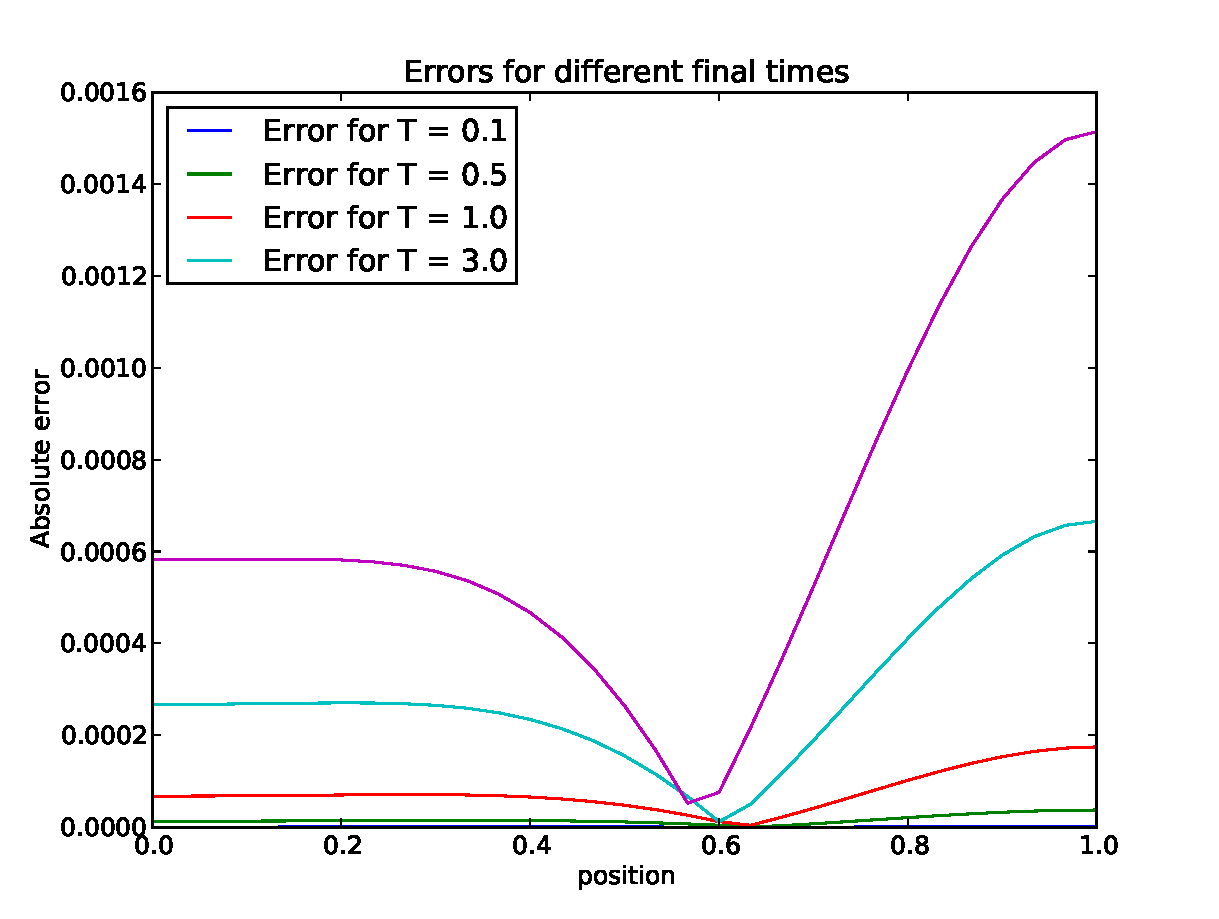
\includegraphics[width=13cm]{errorplot.pdf}
\caption{\label{fig:1} The figure shows the error for different times, using parameters as specified in the text.}
\end{figure}


\section{Sources of errors in the solution}
There are several important sources of errors, notably
\begin{itemize}
 \item We use $\alpha(u^{n-1})$ instead of $\alpha(u^n)$ in our calculations of $a(u,v)$. This could be improved for instance by using several Piccard iterations.
 
 \item Truncation error from approximating the function with piecewise linear elements.

 \item Other sources such as error due to the numerical integration in FEniCS, etc, these should be considered minor.
 
 \item The time discretisation is also a source of error, however this is not explicitly due to FEniCS. 
 \end{itemize}

 \subsection{Elimination of the error due to a single Piccard iteration}
In this section, we will choose $f$ such that our choice for $u$ fulfills equation \eqref{eq:master} with $\alpha(u^{n-1})$ rather than $\alpha(u^n)$. This will eliminate a major source of error, and will allow us to perform a convergence rate test for the manufactured solution. For this case, one can show that $f(x,t)= \rho x^2(-2x + 3)/6 -
(-12tx + 3t(-2x + 3))(x^4(-dt + t)^2(-2x + 3)^2 + 36)/324
- (-6tx^2 + 6tx(-2x + 3))(36x^4(-dt + t)^2(2x - 3)
+ 36x^3(-dt + t)^2(-2x + 3)^2)/5832$, and if we select the same parameters as we did previously, we find errors as shown in table \ref{tab:2}, and a convergence test as performed previously gives the result
\begin{verbatim}
 user@UNIX:~/../prosjekt$ python nonlinear_diffusion.py
 ...
 [1.9583957954613822, 1.9612382435719218, 1.980102551522378, 
 1.981220449666488, 1.988819119920602, 1.9914942289734918]
\end{verbatim}
which again appears to converge.

 \begin{table}[position specifier]
\centering
\begin{tabular}{|c|c|}
\hline
Time & Error \\
\hline
0.1 &  3.20008488e-10    \\
0.5 &   9.51625737e-08  \\
1.0 &   1.33755315e-06   \\
2.0 &   2.05114946e-05 \\
3.0 &   1.04725019e-04 \\
\hline
\end{tabular}
\caption{\label{tab:2}The table shows the total error for different times using the alternate scheme for $f(x,t)$, as described in the text, using parameters as specified in the text. The errors are generally smaller than those in table \ref{tab:1}.}
\end{table}

\section{Nonlinear diffusion of a Gaussian function}
We will now simulate the diffusion of a gaussian function in 2D. Due to symmetry, it suffices to simulate one quarter of the domain:
\begin{equation}
I(x,y)=\exp(−{1 \over 2σ^2} (x^2+y^2)), \quad (x,y)\in \Omega =[0,1]\times[0,1],
\end{equation}
where $\sigma$ measures the width of the Gaussian function. We choose $\alpha(u)=1+\beta u^2$, where $\beta$ is a constant one can play around with.
\subsection{Animating the solution in MayaVI}
The 2D gaussian diffusion is a good cause to explore more powerful animation tools than the standard matplotlib library. MayaVI is a very powerful tool for visualization of 2D-functions, and can be used very similarly to other well known tools such as matplotlib and MATLAB. the function \verb mcrtmv  can be found in the program \verb PDE_tools.py  at www.github.com/andreavs/INF5620/prosjekt/ along with an example in the file \verb diffusion.mpg .

\section{Handling the nonlinear term}
In this section we will look at some other methods of handling the linear term.
\subsection{Group finite element method}
The group finite element method is another way to handle the nonlinear term $\alpha(u)$. In the finite element method we approximate $u^n$ in terms of a set of functions, $u^n = \sum_j c_j^n v_j$. We now assume $\alpha$ is linear in these, so that
\beq
\alpha(u^n) = \alpha \left( \sum_j c_j^n v_j \right) \approx \sum_j \alpha(c_j)v_j.
\eeq
This will assure a linear equation in $u^n$! If we now go back to equation \eqref{eq:inteq}, we can insert the expression for $u^n$ and the group finite element method to get
\begin{equation}
\int_\Omega  \sum_j c_j^n v_j (x)v_i(x) + {\Delta t \over \varrho}\bigg(\sum_j \alpha(c^{n}_j) v_j  \sum_k c_k^n \nabla v_k(x)\cdot \nabla v_i(x) \bigg)\, d\Omega = \int_\Omega (\sum_j c_j^{n-1} v_j(x) + f(x,t^n)) v_i(x) \, d\Omega 
\end{equation}
for all $i$. This can in principle be solved for $c_j^n$, as we have $N$ equations for the $N$ unknowns. 

\subsection{Newtons's method}
Another way to solve for the nonlinear term is to use Newtons method. With $a(u,v)$ and $L(v)$ defined as previously in equations \eqref{eq:a}-\eqref{eq:L}, we can write the problem as 
\begin{align}
 a(u,v) - L(v) = 0 \\
 F(u,v) = 0 \quad \forall v \in V
\end{align}
where $F(u,v) = a(u,v)- L(v)$. If we now insert $u^n = \sum_j c_j^n v_j$. and $v = v_i$, we get the equation
\begin{align}
 F_i(u,v) & = a\left(\sum_j c_j^n v_j, v_i\right) - L(v_i) \\
 & = \int_\Omega  \sum_j c_j^n v_j (x)v_i(x) + {\Delta t \over \varrho}\bigg( \alpha\left(\sum_j c^{n}_j v_j\right)   \sum_k c_k^n \nabla v_k(x)\cdot \nabla v_i(x) \bigg)\, d\Omega  \\
  &-\int_\Omega (\sum_j c_j^{n-1} v_j(x) + f(x,t^n)) v_i(x) \, d\Omega = 0
\end{align}
for all $i$. For such a vector equation, Newtons method can be formulated as 
\begin{align}
 J_F(\textbf{c}_i^n)(\textbf{c}_{i+1}^n - \textbf{c}_{i}^n) = -F(\textbf{c}_i^n)
\end{align}
Which can be iterated and should converge to the correct solution $\textbf{c}^n$, where $J_F$ is the Jacobian for $F$, such that $(J_F)_{ij} = \partial F_i / \partial c_j$. This is a linear system of equations, and in order to solve it, we should calculate $(J_F)_{kl}$. If we note that 
\begin{equation}
{ \partial u \over \partial c_l} = {\partial \over \partial c_l} \sum_j c_j v_j = v_l
\end{equation}
We have that 
\begin{align}
 (J_F)_{kl} & = { \partial F_k \over \partial c_l } \\
 & = \int_\Omega v_k v_l + {\Delta t \over \varrho} \left( {\partial \alpha \over \partial u} \bigg|_{u = u^{n}_i} v_l(x)\sum_j c_j^n \nabla v_j(x)\cdot \nabla v_k(x)  + \alpha(u_i^n) c_l \nabla v_l(x) \cdot \nabla v_k(x) \right) \, d\Omega
\end{align}
If we now reduce the problem to one space dimension and using P1 elements, and integrating with the trapezoidal rule (using the node endpoints as integration points) we have that 
\begin{align}
 \int_\Omega v_k v_l \, d\Omega = {2h \over 3}\delta_{k,l}% + {h \over 6}\delta_{k,l-1}   
\end{align}
which can easily be checked. The other term requires a bit more work. We first note that $(\partial v_j/ \partial x) (\partial v_k/ \partial x) = 0$ unless $j = k$ or $j = k \pm 1$. In these cases we have 
\begin{align}
{\partial v_k \over \partial x} {\partial v_k \over \partial x} = \begin{cases} h^{-2} & \text{if } x_{k-1} \le x < x_{k+1}  \\ 0 & \text{otherwise}\end{cases}
\end{align}
and
\begin{align}
 {\partial v_k \over \partial x} {\partial v_{k\pm1} \over \partial x} = \begin{cases} -h^{-2} & \text{if } x\in[x_k, x_{k\pm 1})  \\ 0 & \text{otherwise}\end{cases}
\end{align}
Using this we may write the sum over $j$ as 
\begin{align}
 \sum_j c_j^n {\partial v_j \over \partial x}{\partial v_k \over \partial x} = \begin{cases} {c_{k}-c_{k-1} \over h^2} & \text{if } x_{k-1} \le x < x_k \\ {c_{k}-c_{k+1} \over h^2} & \text{if } x_{k} \le x < x_{k+1} \\ 0 & \text{otherwise}  \end{cases}
\end{align}
Using this, we note that the full product including the $v_l$ term will have a nonzero integral only if $l = k$ or $l = k\pm 1$. In total, using the trapezoidal rule, we have
\begin{align}
 \int_\Omega {\partial \alpha \over \partial u} \bigg|_{u = u^{n}_i} v_l(x)\sum_j c_j^n \nabla v_j(x)\cdot \nabla v_k(x)\, d\Omega = \begin{cases} \frac{2}{3}\alpha'(u_{k-1})(c_k - c_{k-1}) & \text{if } l=k-1 \\ \frac{1}{3}\alpha'(u_{k})(2c_k - c_{k+1}- c_{k-1}) & \text{if } l=k \\ \frac{2}{3}\alpha'(u_{k-1})(c_k - c_{k+1}) & \text{if } l=k+1 \\ 0 & \text{otherwise} \end{cases}
\end{align}
And finally, from the $\alpha(u) c_l \nabla v_l(x) \cdot \nabla v_k(x)$ term we get 
\begin{align}
 \int_\Omega \alpha(u) c_l \nabla v_l(x) \cdot \nabla v_k(x) \, d\Omega = \begin{cases} -\alpha(u_{k-1})c_{k-1}/h & \text{if } l = k-1 \\ 2\alpha(u_{k})c_{k}/h & \text{if } l = k \\ -\alpha(u_{k+1})c_{k+1}/h & \text{if } l = k+1 \\ 0 & \text{otherwise} \end{cases}
\end{align}
Gathering all the results, we find that 
\begin{align}
 (J_F)_{kl} = \begin{cases} {\Delta t \over \varrho}\left(\frac{2}{3}\alpha'(u_{k-1})(c_k - c_{k-1})  -\alpha(u_{k-1})c_{k-1}/h\right) & \text{if } l = k-1 \\ {2h \over 3} + \frac{1}{3}\alpha'(u_{k})(2c_k - c_{k+1}- c_{k-1}) + 2\alpha(u_{k})c_{k}/h & \text{if } l = k \\ \frac{2}{3}\alpha'(u_{k-1})(c_k - c_{k+1}) -\alpha(u_{k+1})c_{k+1}/h & \text{if } l = k+1 \\ 0 & \text{otherwise}  \end{cases}
\end{align}


\end{document}

